\section{环境搭建}

\begin{frame}[fragile]{第一个程序}
\begin{columns}[T,onlytextwidth]
\column{0.50\textwidth}
\begin{block}{源代码}
\small\begin{lstlisting}[language=c]
#include <stdio.h>
int main() {
    printf("Hello, world!\n");
}
\end{lstlisting}
\end{block}

\column{0.05\textwidth}
\begin{block}{}\end{block}
\begin{block}{->}\end{block}
\begin{block}{}\end{block}

\column{0.30\textwidth}
\begin{block}{执行结果}
\small\begin{lstlisting}
Hello, world!
\end{lstlisting}
\end{block}
\end{columns}

\begin{itemize}[<+- | alert@+>]
\item C源代码是如何变成 exe 文件的呢?
\item 编译
\end{itemize}
\end{frame}

\begin{frame}[fragile]{如何编译C源代码?}
\begin{itemize}[<+- | alert@+>]
\item 需要一个编译器
\item 常见的编译器: GCC, CLANG, MSVC
\item 以GCC为例, 编译并执行main.c
\begin{verbatim}
  gcc main.c -o main
  ./main
\end{verbatim}
\item 代码用什么修改? VIM? EMACS?
\item 改了代码再编译呢? 重新敲一遍? 写个脚本或Makefile?
\item 出BUG了,怎么调试呢? 听说可以用GDB?
\item \sout{可是vim, gcc, make, gdb我都不会啊}
\item 你需要一个集成开发环境(IDE)
\end{itemize}
\end{frame}

\begin{frame}[fragile]{集成开发环境}
VS和CLion都很优秀, 这里有安装教程:
\href{http://problemoverflow.top/c/0.%E5%BC%80%E5%8F%91%E7%8E%AF%E5%A2%83%E6%90%AD%E5%BB%BA/0.0.Microsoft_Visual_Studio.html}{VS},
\href{http://problemoverflow.top/c/0.%E5%BC%80%E5%8F%91%E7%8E%AF%E5%A2%83%E6%90%AD%E5%BB%BA/0.1.CLion.html}{CLion}

CLion相比于VS有许多\href{http://problemoverflow.top/index.php?qa=33&qa_1=%E6%89%80%E4%BB%A5%E5%88%B0%E5%BA%95%E7%94%A8%E4%BB%80%E4%B9%88-ide-%E5%86%99-oj%EF%BC%9F&show=36#a36}{优点}
\begin{itemize}
\item 使用跨平台的CMAKE管理工程
\item 编辑器提示更智能
\item 可高度定制等
\end{itemize}
如果还没有安装CLion, 请下载: \href{https://www.jetbrains.com/clion/download}{CLion}, \href{https://nchc.dl.sourceforge.net/project/mingw-w64/Toolchains%20targetting%20Win64/Personal%20Builds/mingw-builds/8.1.0/threads-posix/seh/x86_64-8.1.0-release-posix-seh-rt_v6-rev0.7z}{MinGW}
\end{frame}

\begin{frame}[fragile]{CLion快速配置}
\href{https://nchc.dl.sourceforge.net/project/mingw-w64/Toolchains%20targetting%20Win64/Personal%20Builds/mingw-builds/8.1.0/threads-posix/seh/x86_64-8.1.0-release-posix-seh-rt_v6-rev0.7z}{MinGW} (提供make, gcc, g++, gdb):

解压缩 \href{https://nchc.dl.sourceforge.net/project/mingw-w64/Toolchains%20targetting%20Win64/Personal%20Builds/mingw-builds/8.1.0/threads-posix/seh/x86_64-8.1.0-release-posix-seh-rt_v6-rev0.7z}{x86\_64-8.1.0-release-posix-seh-rt\_v6-rev0.7z} 到任意目录

\emptyline
\href{https://www.jetbrains.com/clion/download}{CLion} (IDE):

安装 \href{https://www.jetbrains.com/clion/download}{CLion-2019.2.4.exe}, 打开 CLion 设置, 将刚才的解压目录填入红框
\begin{figure}[ht!]
\centering
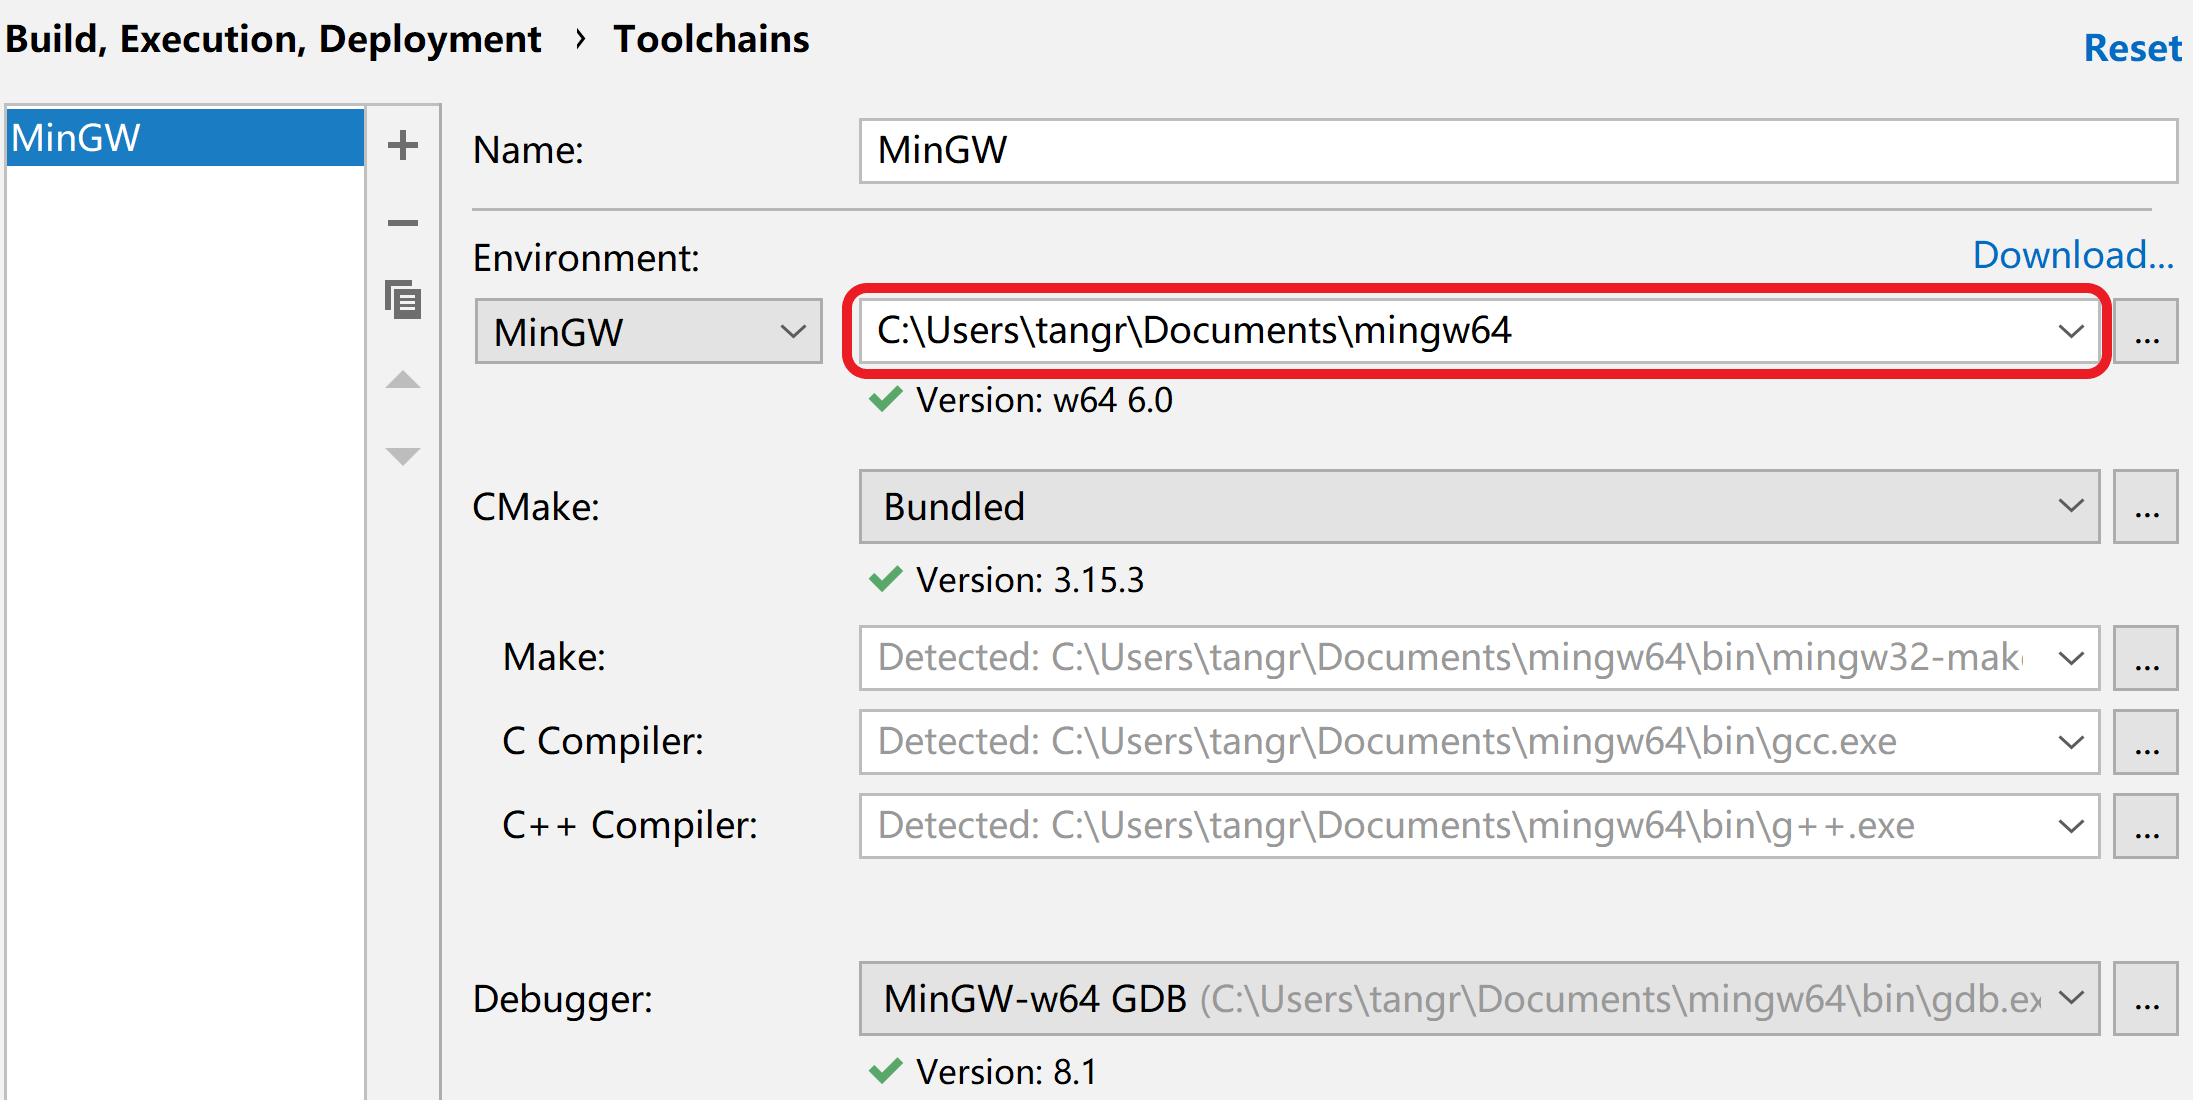
\includegraphics[width=75mm]{figs/clion_mingw.png}
\caption{CLion 配置MinGW}
\end{figure}
\end{frame}

\begin{frame}[fragile]{自定义 CMakeLists.txt}
下载 \href{http://problemoverflow.top/download/OJ.zip}{http://problemoverflow.top/download/OJ.zip}

解压并用CLion打开该目录, 打开 CMakeLists.txt

\emptyline

部分解释:
\begin{itemize}[<+- | alert@+>]

\item 第4-5行: 定义使用的标准为C99和C++11 (符合OJ设置)

\item 第7行: 使编译器产生更多警告, 并将警告视为错误 (比OJ严格)

\item 第8行: 定义了一个宏\texttt{DEBUG}, 用于 redirect.h (后面讲, 不影响OJ)

\item 第9行: math.h需要链接的数学函数库 (符合OJ设置)

\item 第11-22行: 定义多个可执行文件设置, 方便管理
\end{itemize}

\end{frame}


\begin{frame}[fragile]{输入输出重定向}
\begin{itemize}[<+- | alert@+>]
\item 调试OJ时, 一个很烦的事情是每次都需要重新输入

\item 程序员最讨厌重复劳动. 如何解决这个问题? 

\item 如果你用的是Linux, 一个很简单的方法就是输入重定向:
\begin{verbatim}
  ./sum <input.txt
  echo 1 2 3 | ./sum
\end{verbatim}

\item 但在用CLion的时候输入命令行仍然很麻烦
\item redirect.h 解决了这个问题
\begin{itemize}
\item 不提供输入文件时从命令行窗口读取用户输入
\item 提供输入文件时通过输入文件读取输入
\item 提供输出文件时输出到该文件
\end{itemize}
\end{itemize}
\end{frame}

\begin{frame}[fragile]{输入输出重定向}
\begin{itemize}[<+- | alert@+>]
\item 代码编写样例见 main.c
\item 命令行: \texttt{./main [input] [output]}  (中括号为可选)
\item 在Program arguments中添加 \texttt{../input/1-1-a\_sum.txt}
\emptyline\begin{figure}[ht!]
\centering
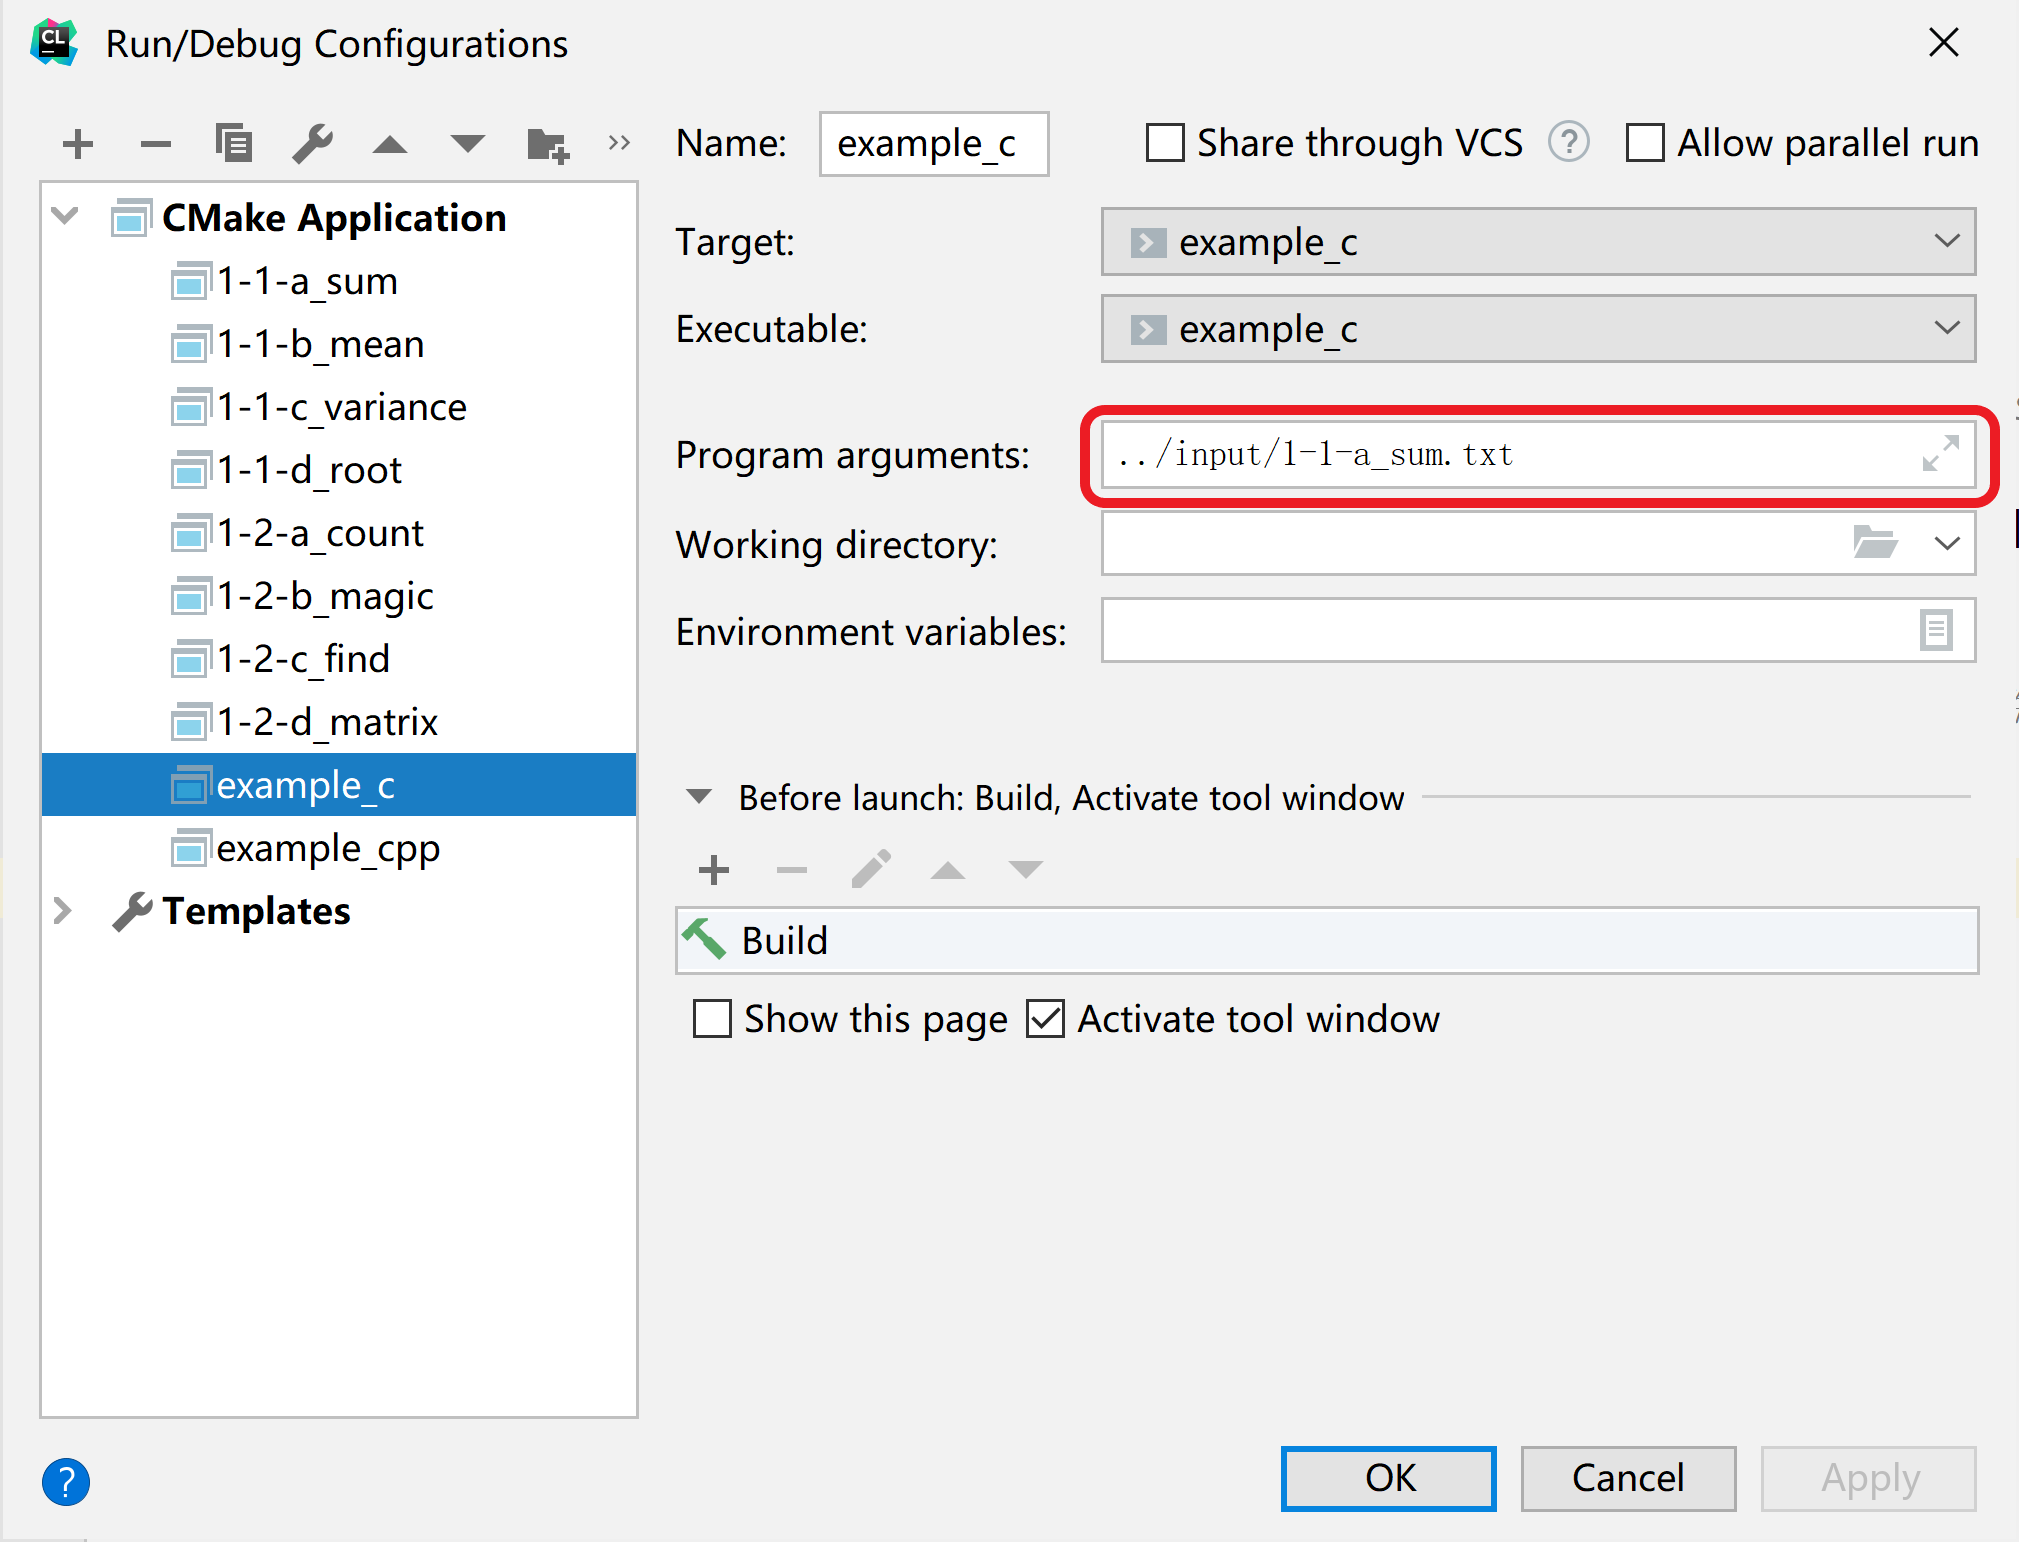
\includegraphics[width=65mm]{figs/clion_cmdargs.png}
\caption{CLion 添加命令行参数}
\end{figure}
\end{itemize}
\end{frame}
